\documentclass[compress,aspectratio=43]{beamer}
\usepackage[latin1]{inputenc}
\usepackage{tikz}
\usepackage{xcolor}
\usepackage{amsmath,amssymb,epsfig,graphicx,url,bbm,epstopdf}

%\usetheme{Szeged}
\useoutertheme[subsection=false, footline=institutetitle]{miniframes}
\usecolortheme{beaver}

\setbeamercolor{subtitle}{fg=black} % Change subtitle color
\setbeamercolor{block title}{fg=black} % Change subtitle color
\setbeamercolor{itemize item}{fg=red}
\setbeamercolor{itemize itemize}{fg=red}


\setbeamertemplate{navigation symbols}{}%remove navigation symbols
\definecolor{darkgreen}{rgb}{0,0.5,0}

% Footer
\makeatletter
\setbeamertemplate{footline}
{
  \leavevmode%
  \hbox{%
  \begin{beamercolorbox}[wd=.333333\paperwidth,ht=2.25ex,dp=1ex,left]{section in head/foot}%
    \usebeamerfont{author in head/foot}\insertshortauthor
  \end{beamercolorbox}%
  \begin{beamercolorbox}[wd=.333333\paperwidth,ht=2.25ex,dp=1ex,center]{section in head/foot}%
    \usebeamerfont{title in head/foot}\insertshorttitle
  \end{beamercolorbox}%
  \begin{beamercolorbox}[wd=.333333\paperwidth,ht=2.25ex,dp=1ex,right]{section in head/foot}%
    \usebeamerfont{date in head/foot}\insertshortdate{}\hspace*{2em}
    \insertframenumber{} / \inserttotalframenumber\hspace*{2ex} 
  \end{beamercolorbox}}%
  \vskip0pt%
}
\makeatother

\usebackgroundtemplate{%
	\tikz\node[opacity=0.05] {
\includegraphics[height=500px,width=500px]{stanford_seal.png}};
}

% Removes title background bar
\setbeamercolor*{frametitle}{bg=}
\setbeamercolor{titlelike}{parent=structure}

\title[Stanford University]{Object Detection with R-CNN}
\subtitle{\scriptsize \vspace{3mm}Ross Girshick, Jeff Donahue, Trevor Darrell, and Jitendra Malik\\University of California, Berkeley\vspace{-3mm}}
\author[\enspace\,\,\, Albert Haque, Fahim Dalvi]{
{\scriptsize Project Presentation By}\\
Albert Haque and Fahim Dalvi
}
\institute[Stanford University]{}
\date{June 3, 2015}
\begin{document}

\section{}% Top left running header
\begin{frame}
\titlepage
\end{frame}

\begin{frame}{Outline}
\begin{itemize}
\item{Baseline Results}
    \begin{itemize}
        \item Iterative SVM
        \item Full SVM
    \end{itemize} 
    \item{Extensions}
    \begin{itemize}
        \item SGD based implementation
        \item VGG Network
    \end{itemize}
\end{itemize}
\end{frame}

\begin{frame}{Baseline Results}
\only<1> {
    \begin{itemize}
    \item Setup
        \begin{itemize}
            \item Validation set (100 images)
            \item Zero-mean unit-variance normalization
            \item $\ell_2$ regularization loss
            \item Number of negatives: 30,000 for iterative SVM
            \item Positives weighted 10 times more than negatives
        \end{itemize}
    \item Results
        \begin{itemize}
        \item Full SVM gives no improvement over Iterative SVM
        \item 65\% accuracy on the validation set
        \end{itemize}
    \end{itemize}
}
\only<2> {
    \begin{figure}
		\centering
		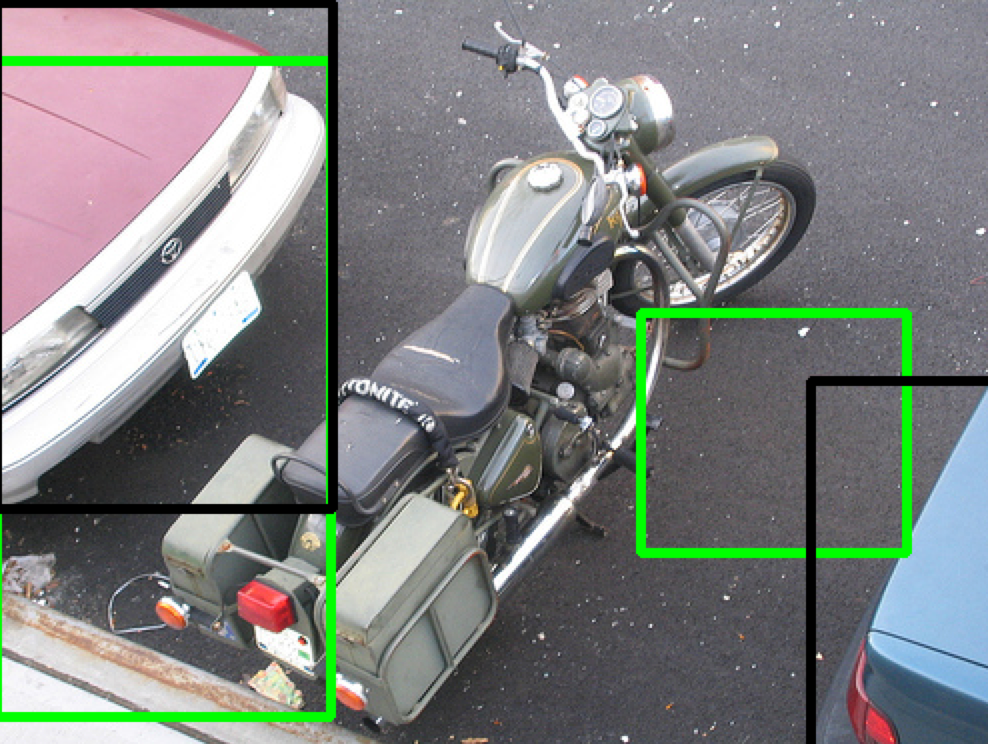
\includegraphics[width=0.3\textwidth]{figures/baseline/example1.png}
		\hspace{2mm}
		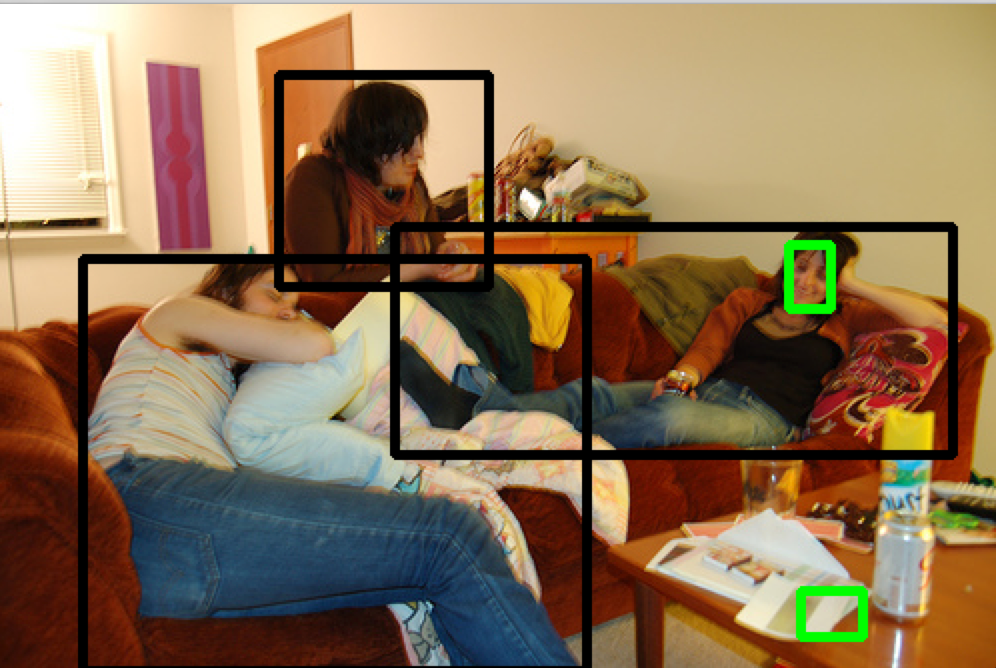
\includegraphics[width=0.3\textwidth]{figures/baseline/example2.png}
		\hspace{2mm}
		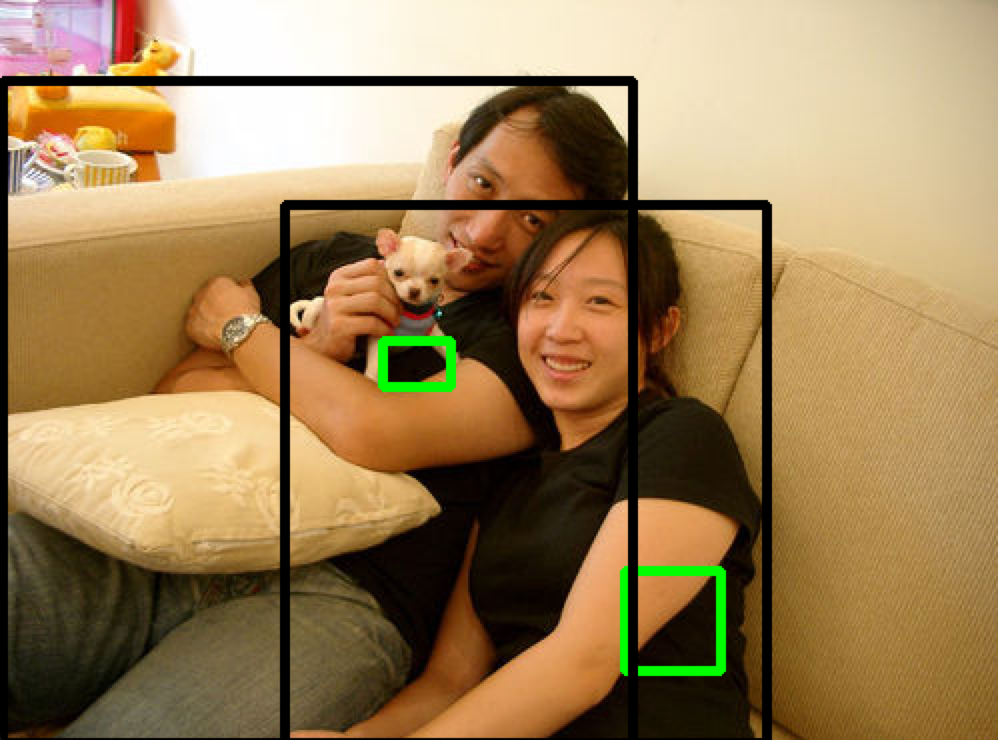
\includegraphics[width=0.3\textwidth]{figures/baseline/example3.png}\\
		\vspace{3mm}
		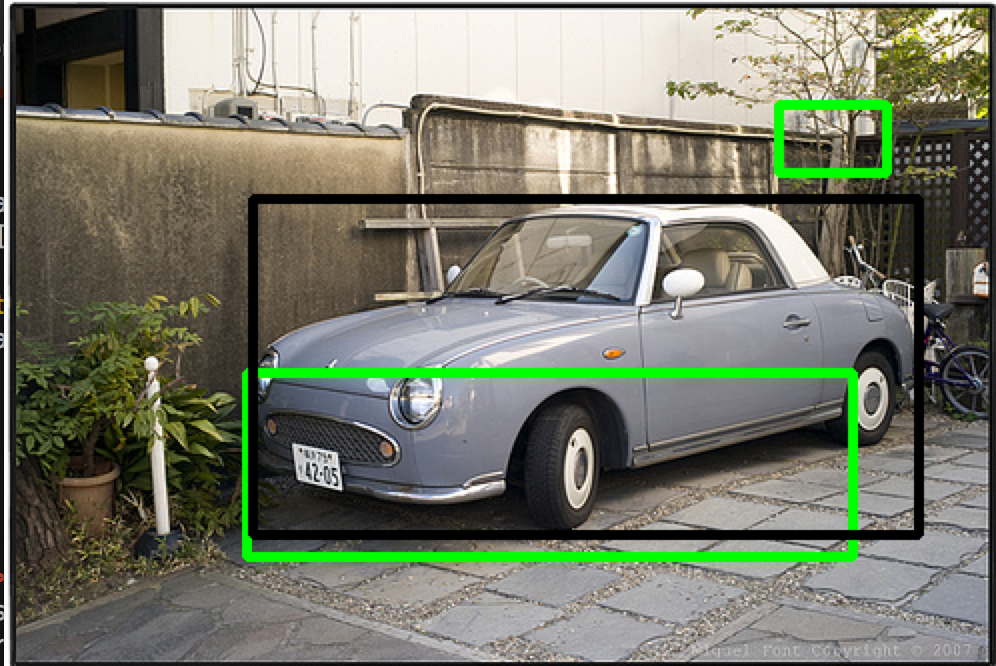
\includegraphics[width=0.3\textwidth]{figures/baseline/example4.png}
		\hspace{2mm}
		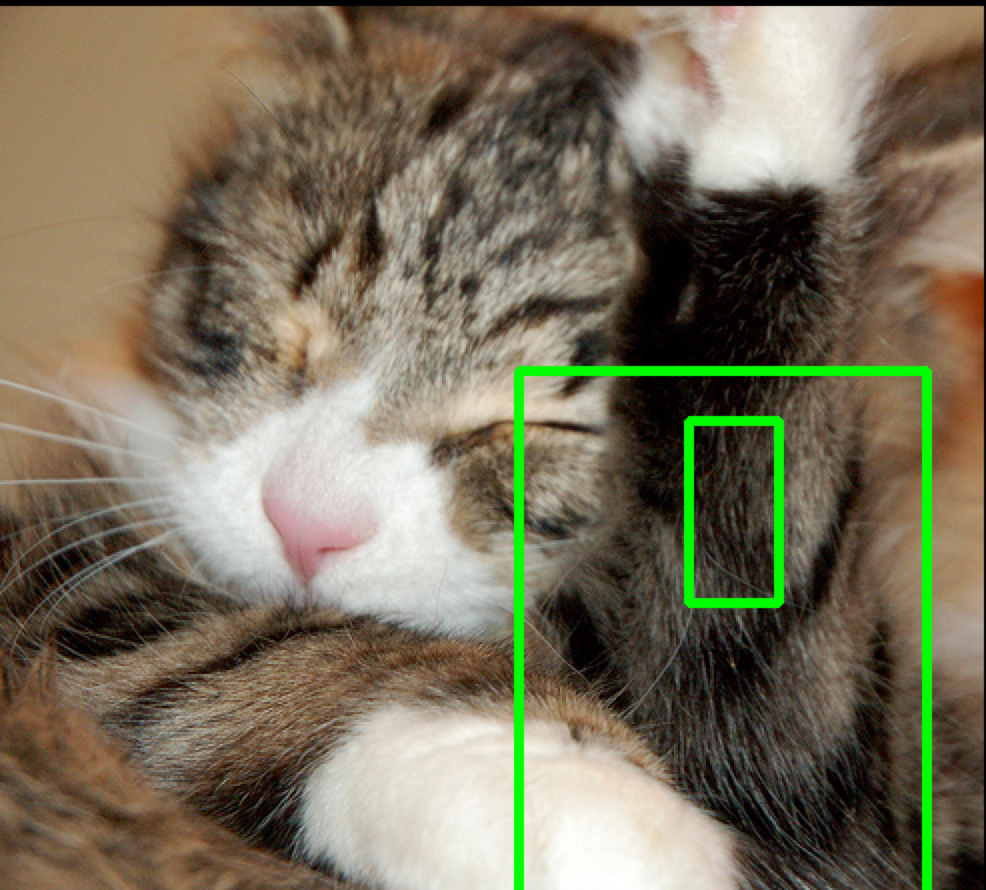
\includegraphics[width=0.3\textwidth]{figures/baseline/example5.png}
		\hspace{2mm}
		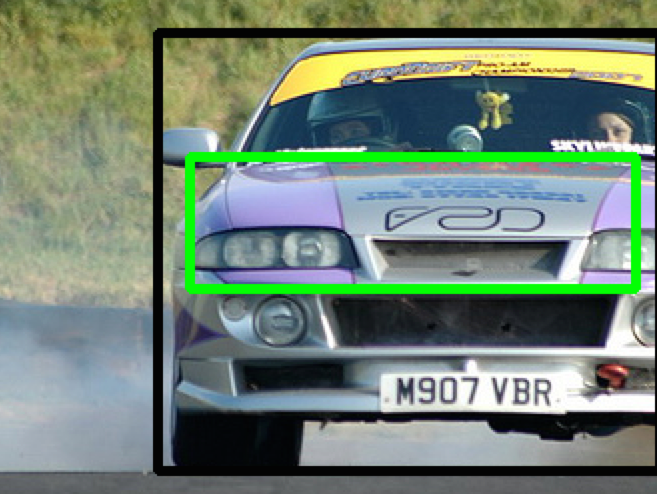
\includegraphics[width=0.3\textwidth]{figures/baseline/example6_cropped.png}
	\end{figure}
}
\only<3> {
    \begin{figure}
		\centering
		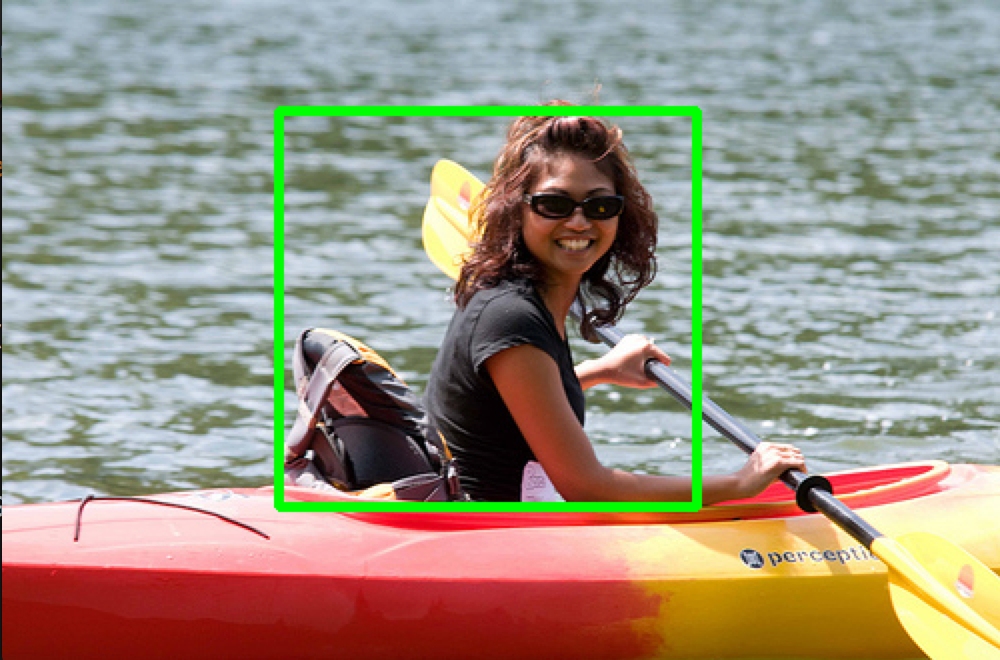
\includegraphics[width=0.7\textwidth]{figures/baseline/example7.png}
	\end{figure}
}
\end{frame}

\begin{frame}{Extensions}
\only<1> {
    \begin{itemize}
    \item SGD Classifier
        \begin{itemize}
            \item Trained iteratively using small sets of images
            \item Same setup as SVM
        \end{itemize}
    \item Results
        \begin{itemize}
        \item SGD classifier does half as worse as the SVM
        \item 55\% accuracy on the validation set
        \end{itemize}
    \end{itemize}
}
\only<2> {
    \begin{columns}
        \begin{column}{0.3\textwidth}
    		\centering
    		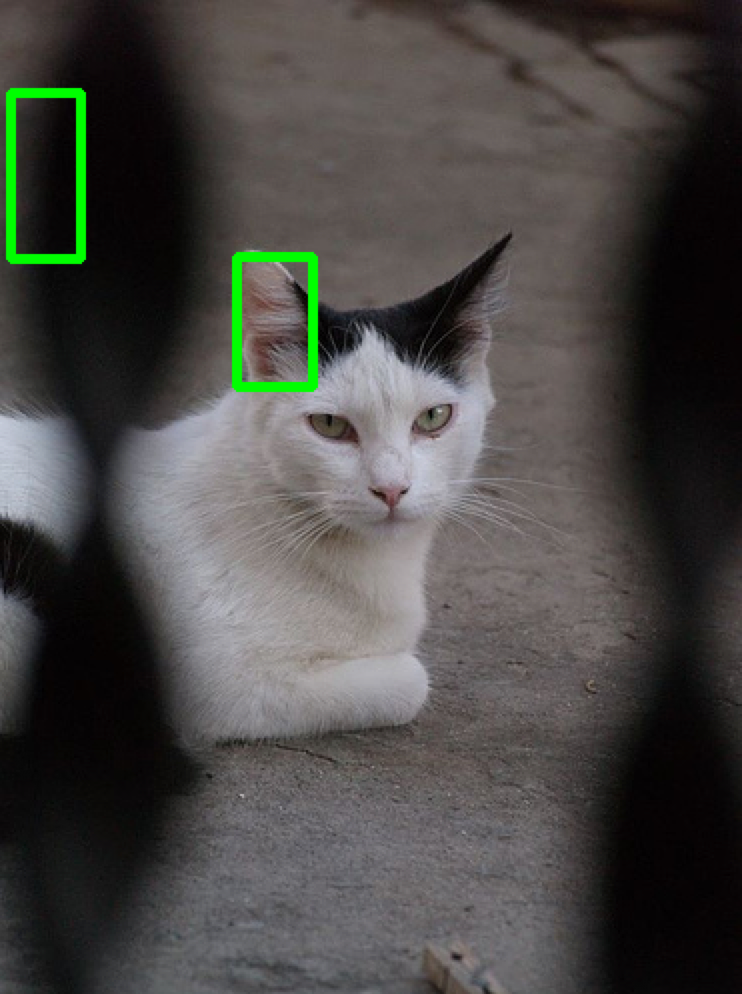
\includegraphics[width=1\linewidth]{figures/sgd/car.png} \\
    		{\scriptsize Car}
		\end{column}
		\begin{column}{0.3\textwidth}
		    \hspace{2mm}
    		\centering
    		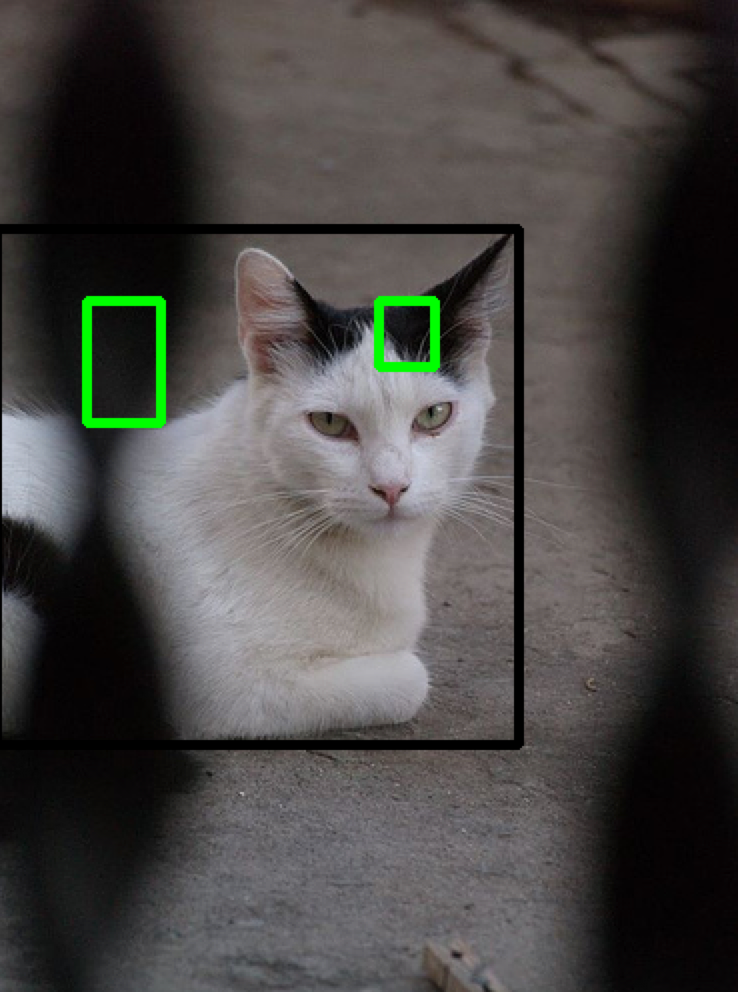
\includegraphics[width=1\linewidth]{figures/sgd/cat.png} \\
    		{\scriptsize Cat}
		\end{column}
		\begin{column}{0.3\textwidth}
    		\hspace{2mm}
    		\centering
    		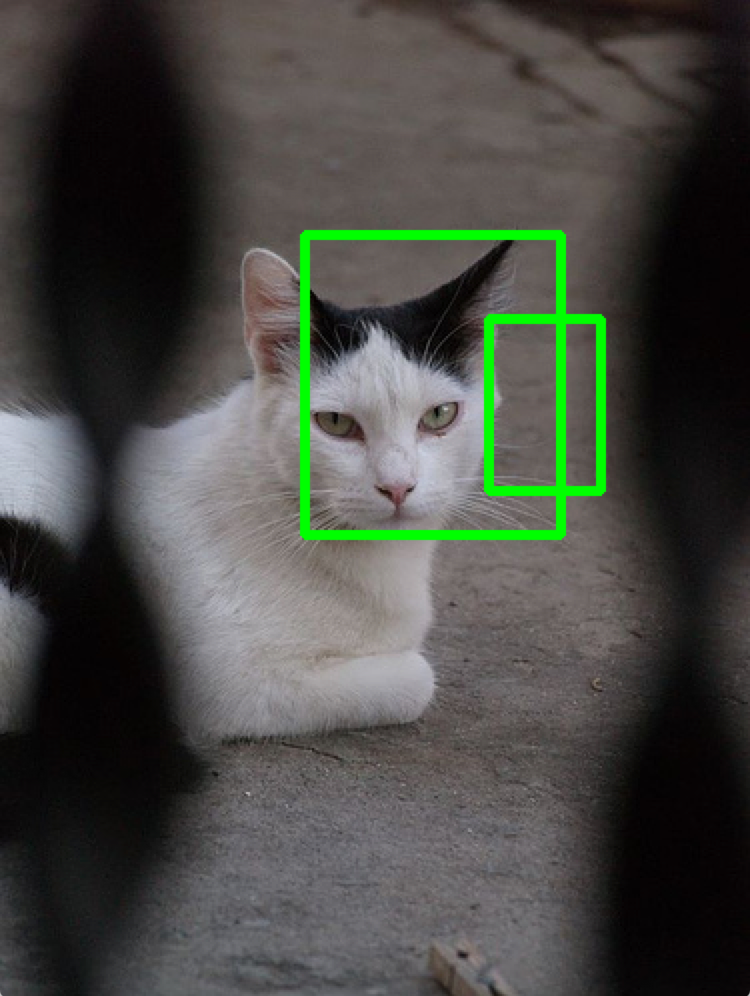
\includegraphics[width=1\linewidth]{figures/sgd/person.png} \\
    		{\scriptsize Person}
		\end{column}
	\end{columns}
}
\end{frame}

\begin{frame}{Extensions}
\only<1> {
    \begin{itemize}
    \item VGG Network
        \begin{itemize}
            \item Features extraction is complete (6 hours on 20 GPUs)
            \item Currently using fc7 non-rectified features
            \item SVM training is in progress
        \end{itemize}
    \end{itemize}
}
\end{frame}

\end{document}